\PassOptionsToPackage{unicode}{hyperref}
\documentclass[aspectratio=1610, 9pt]{beamer}

% Load packages you need here
%\usepackage{polyglossia}
%\setmainlanguage{german}

\usepackage{csquotes}

\usepackage{amsmath}
\usepackage{amssymb}
\usepackage{mathtools}

\usepackage{braket}
\usepackage{graphicx}

\usepackage{hyperref}
\hypersetup{
  linkcolor= {tudark}, % internal links
  citecolor={tugreen}, % citations
  urlcolor={tudark} % external links/urls
  }
\usepackage{bookmark}

\usepackage[english]{babel}
\usepackage[
backend=biber,
style=authoryear-comp
]{biblatex}

\bibliography{lit.bib}

\usepackage{siunitx}
\usepackage{multicol}

\usepackage{booktabs}

\definecolor{light-gray}{HTML}{b0b5b0}

% load the theme after all packages

\usetheme[
  showtotalframes, % show total number of frames in the footline
]{tudo}

% Put settings here, like
\unimathsetup{
  math-style=ISO,
  bold-style=ISO,
  nabla=upright,
  partial=upright,
  mathrm=sym,
}

\title{Maskenerkennung}
\author[L.~Kolk,~J.~Blank]{Lars Kolk\\ Jonah Blank}
\institute[ML-Seminar]{\\[0.3cm]TU Dortmund \\ \Large ML-Seminar}

\begin{document}

\maketitle


\begin{frame}{Fragestellung}
\begin{itemize}
  \item Grundlegende Fragestellung:
  \item ``Kann ein neuronales Netz erkennen, ob eine Person eine Maske trägt?''
  \vspace{0.5cm}
  \item Inhalt
  \begin{itemize}
    \item Datensatz
    \item Datenaufbereitung
    \item Fully Connected Network vs Convolutional Network
    \item Aussicht
\end{itemize}
\end{itemize}
\end{frame}


\begin{frame}{Datensatz}
  \begin{columns}
    \begin{column}{0.48\textwidth}
      \begin{itemize}
        \item Quelle: \href{https://www.kaggle.com/wobotintelligence/face-mask-detection-dataset/data}{Kaggle}
        \item Lizenz: Public Domain (CC0)
        \item $6024$ Bilder \textrightarrow $7271$ Gesichter
        \item 4 Oberklassen:
        \begin{itemize}
          \item face\_no\_mask: 0
          \item face\_other\_covering: 1
          \item face\_with\_mask: 2
          \item face\_with\_mask\_incorrect: 3
        \end{itemize}
        \end{itemize}
    \end{column}
    \begin{column}{0.48\textwidth}
      \begin{figure}
        \centering
        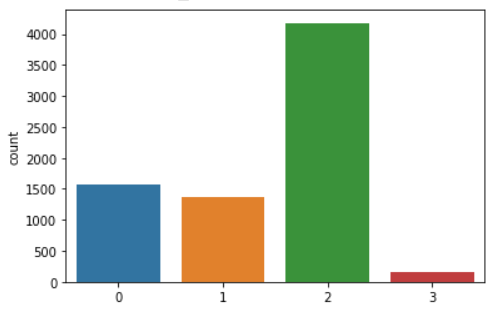
\includegraphics[width = 0.8\textwidth]{images/Verteilung.png}
      \end{figure}
    \end{column}
  \end{columns}
\end{frame}

\begin{frame}{Datenaufbereitung}
  \begin{columns}
    \begin{column}{0.48\textwidth}
      \begin{itemize}
        \item Schneide Bilder auf Gesichter zu
        \item Bringe alle Bilder auf die gleiche Größe
        \begin{itemize}
          \item $50 \times 50$ Pixel
        \end{itemize}
        \item Berechne Matrizen der Bilder
        \item Wende MinMaxScalar an
      \end{itemize}
    \end{column}
    \begin{column}{0.48\textwidth}
      \begin{figure}
        \centering
        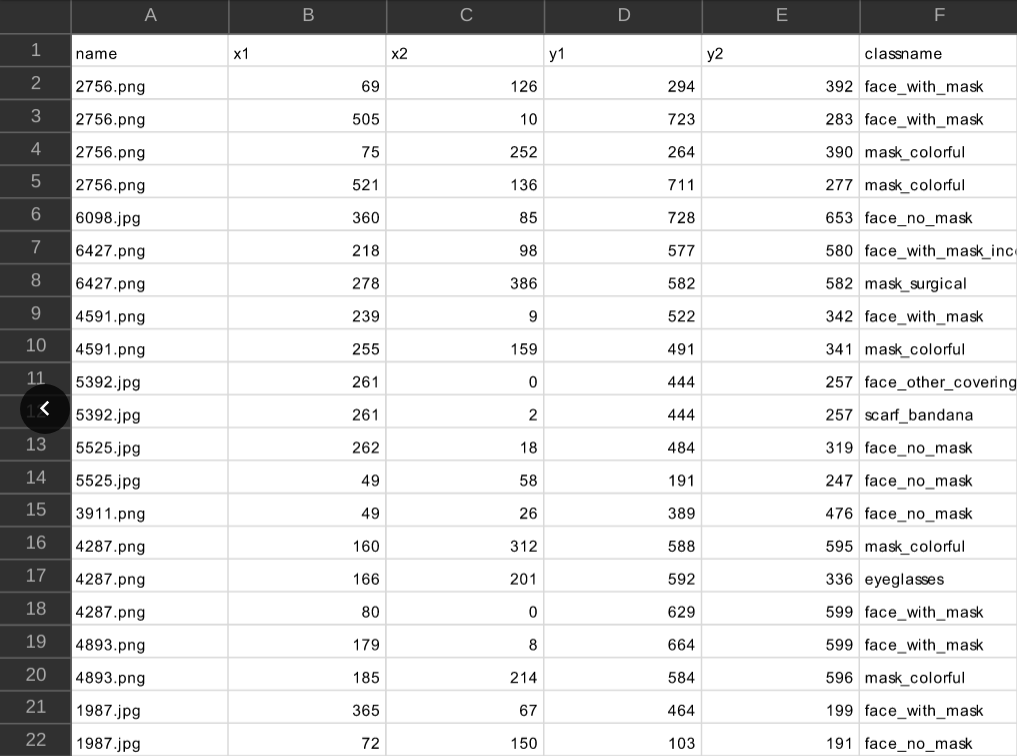
\includegraphics[width = 0.8\textwidth]{images/Datensatz.png}
      \end{figure}
    \end{column}
  \end{columns}
\end{frame}

\begin{frame}{Fully Connected Network}
  \begin{columns}
    \begin{column}{0.48 \textwidth }
      \begin{figure}
        \centering
        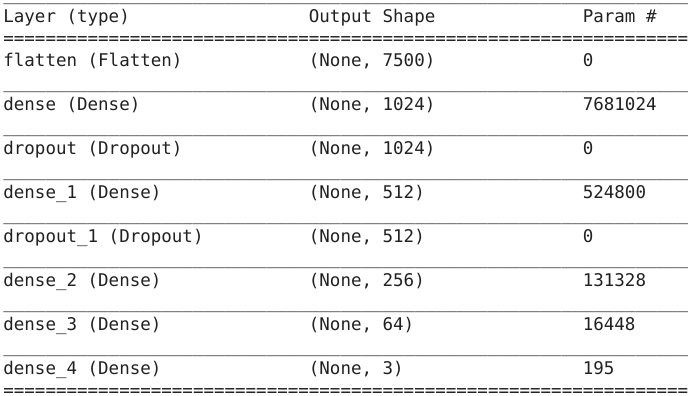
\includegraphics[width = 0.8\textwidth]{images/NN.png}
      \end{figure}
      \begin{itemize}
        \item []dropout = $0.2$
      \end{itemize}
    \end{column}
    \begin{column}{0.48 \textwidth }
      \centering
      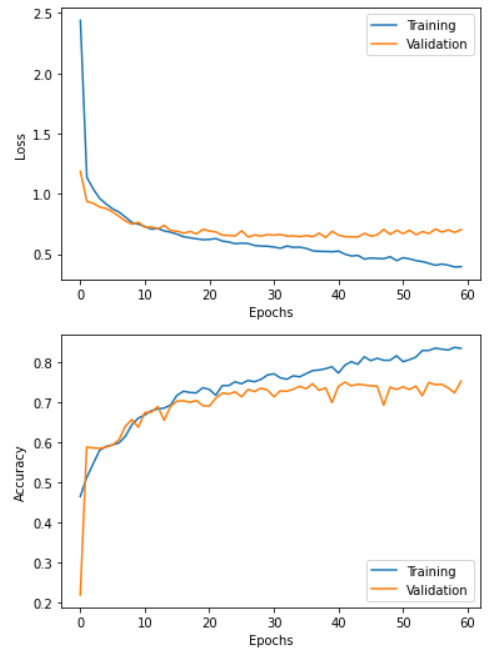
\includegraphics[width = 0.8\textwidth]{images/History.png}
    \end{column}
  \end{columns}
\end{frame}

\begin{frame}
  \begin{columns}
    \begin{column}{0.3 \textwidth }
      \begin{figure}
        \centering
        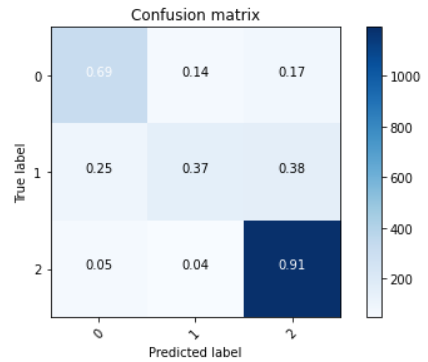
\includegraphics[width = 0.8\textwidth]{images/Matrix.png}
      \end{figure}
    \end{column}
    \begin{column}{0.7 \textwidth }
      \centering
      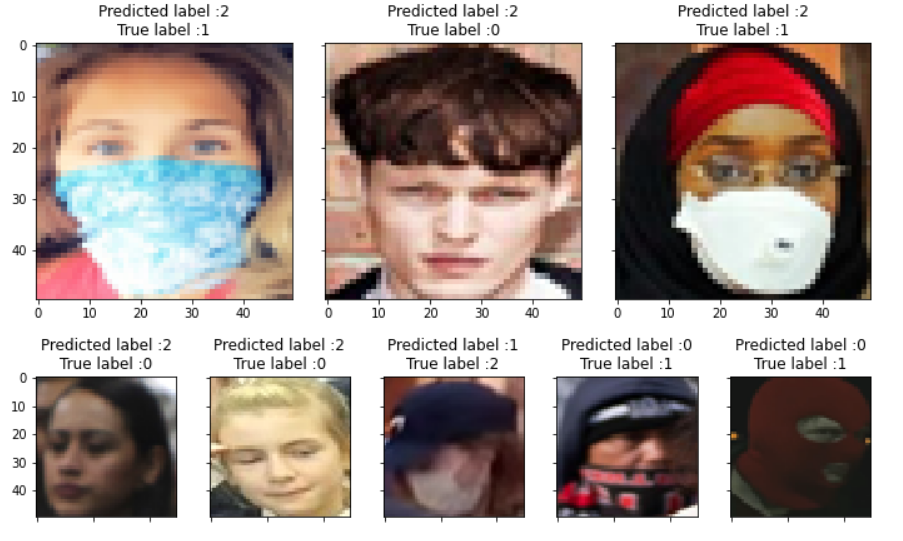
\includegraphics[width = 0.8\textwidth]{images/Bilder.png}
    \end{column}
  \end{columns}
\end{frame}

\begin{frame}{Convolutional Neural Network}
  \begin{figure}
    \centering
    \begin{minipage}{\textwidth}
      \includegraphics[height=0.4\textheight]{images/grid.png}
    \end{minipage}
    \uncover<2>{
      \begin{minipage}{\textwidth}
        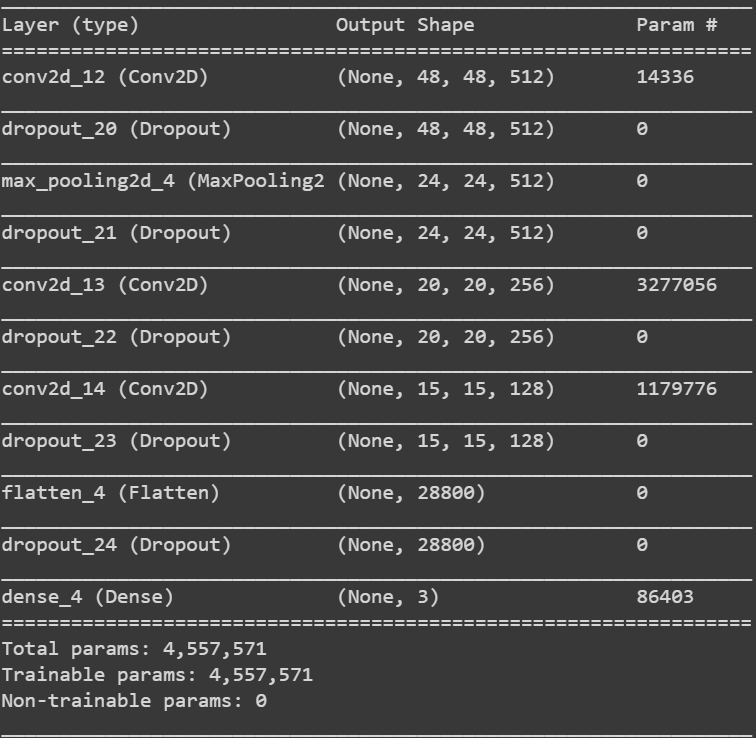
\includegraphics[height=0.55\textheight]{images/CNN.png}
      \end{minipage}
    }
  \end{figure}
\end{frame}

\begin{frame}
  \begin{figure}
    \centering
    \begin{minipage}{0.46\textwidth}
      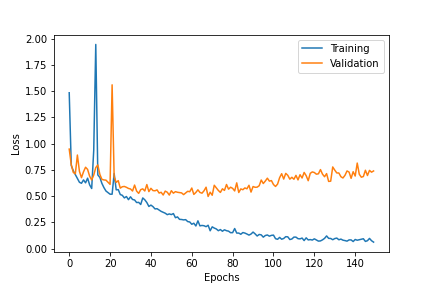
\includegraphics[width=0.85\textwidth]{images/loss.png}
    \end{minipage}
    \begin{minipage}{0.46\textwidth}
      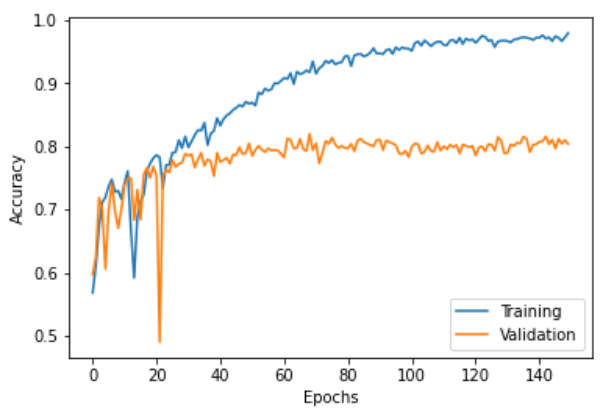
\includegraphics[width=0.85\textwidth]{images/acc.png}
    \end{minipage}
  \end{figure}
\end{frame}

\begin{frame}
  \begin{figure}
  \begin{minipage}{\textwidth}
    \centering
    \begin{minipage}{0.4\textwidth}
      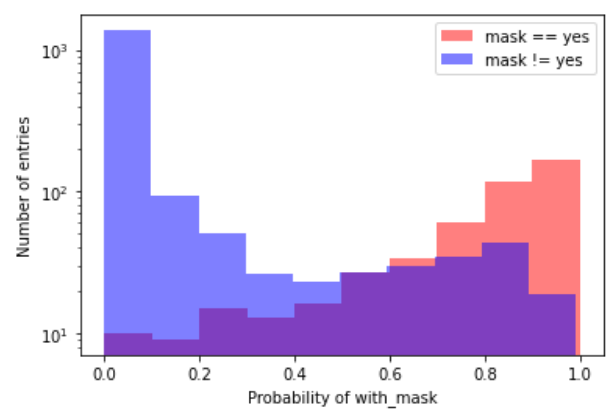
\includegraphics[width=0.85\textwidth]{images/mask.png}
    \end{minipage}
    \begin{minipage}{0.4\textwidth}
      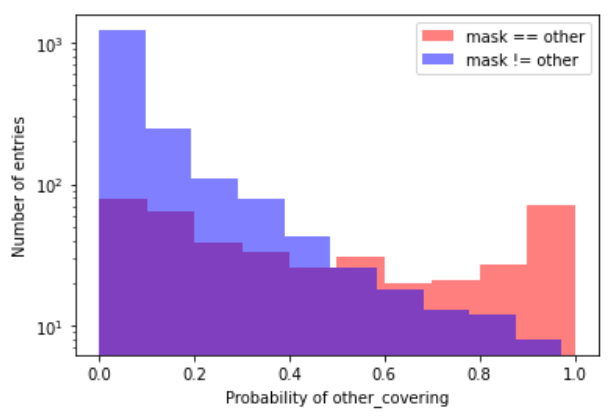
\includegraphics[width=0.85\textwidth]{images/other.png}
    \end{minipage}
  \end{minipage}
  \begin{minipage}{\textwidth}
    \centering
    \begin{minipage}{0.4\textwidth}
      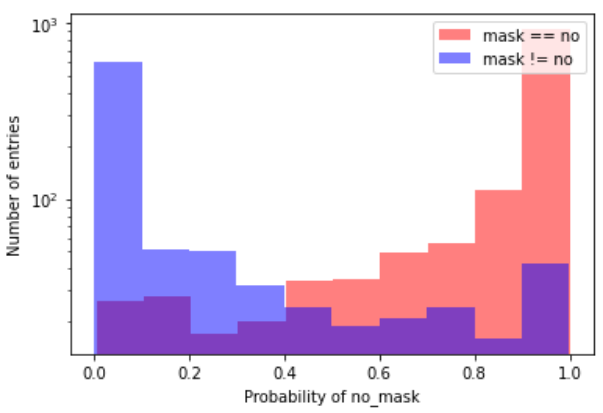
\includegraphics[width=0.85\textwidth]{images/nomask.png}
    \end{minipage}
    \begin{minipage}{0.4\textwidth}
      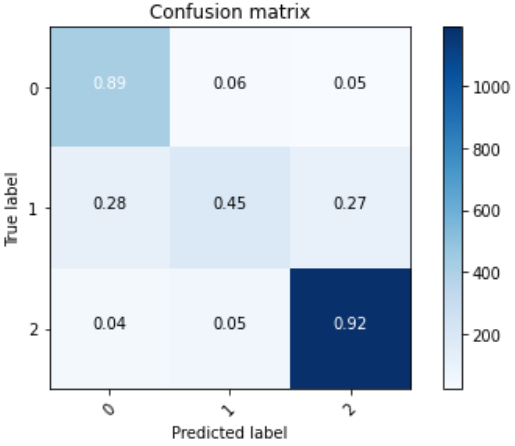
\includegraphics[width=0.8\textwidth]{images/conf.png}
    \end{minipage}
  \end{minipage}
  \end{figure}
\end{frame}

\end{document}
